%	http://www.texample.net/tikz/examples/seismic-focal-mechanism-in-3d-view/
\documentclass[tikz,11pt]{standalone}
\usepackage{tikz-3dplot}
%%%%%%%%%%%
%% helper macros
%: Styles for XYZ-Coordinate Systems
%: isometric  South West : X , South East : Y , North : Z
\tikzset{isometricXYZ/.style={x={(-0.866cm,-0.5cm)}, y={(0.866cm,-0.5cm)}, z={(0cm,1cm)}}}

%: isometric South West : Z , South East : X , North : Y
\tikzset{isometricZXY/.style={x={(0.866cm,-0.5cm)}, y={(0cm,1cm)}, z={(-0.866cm,-0.5cm)}}}

%: isometric South West : Y , South East : Z , North : X
\tikzset{isometricYZX/.style={x={(0cm,1cm)}, y={(-0.866cm,-0.5cm)}, z={(0.866cm,-0.5cm)}}}

%% document-wide tikz options and styles
\begin{document}
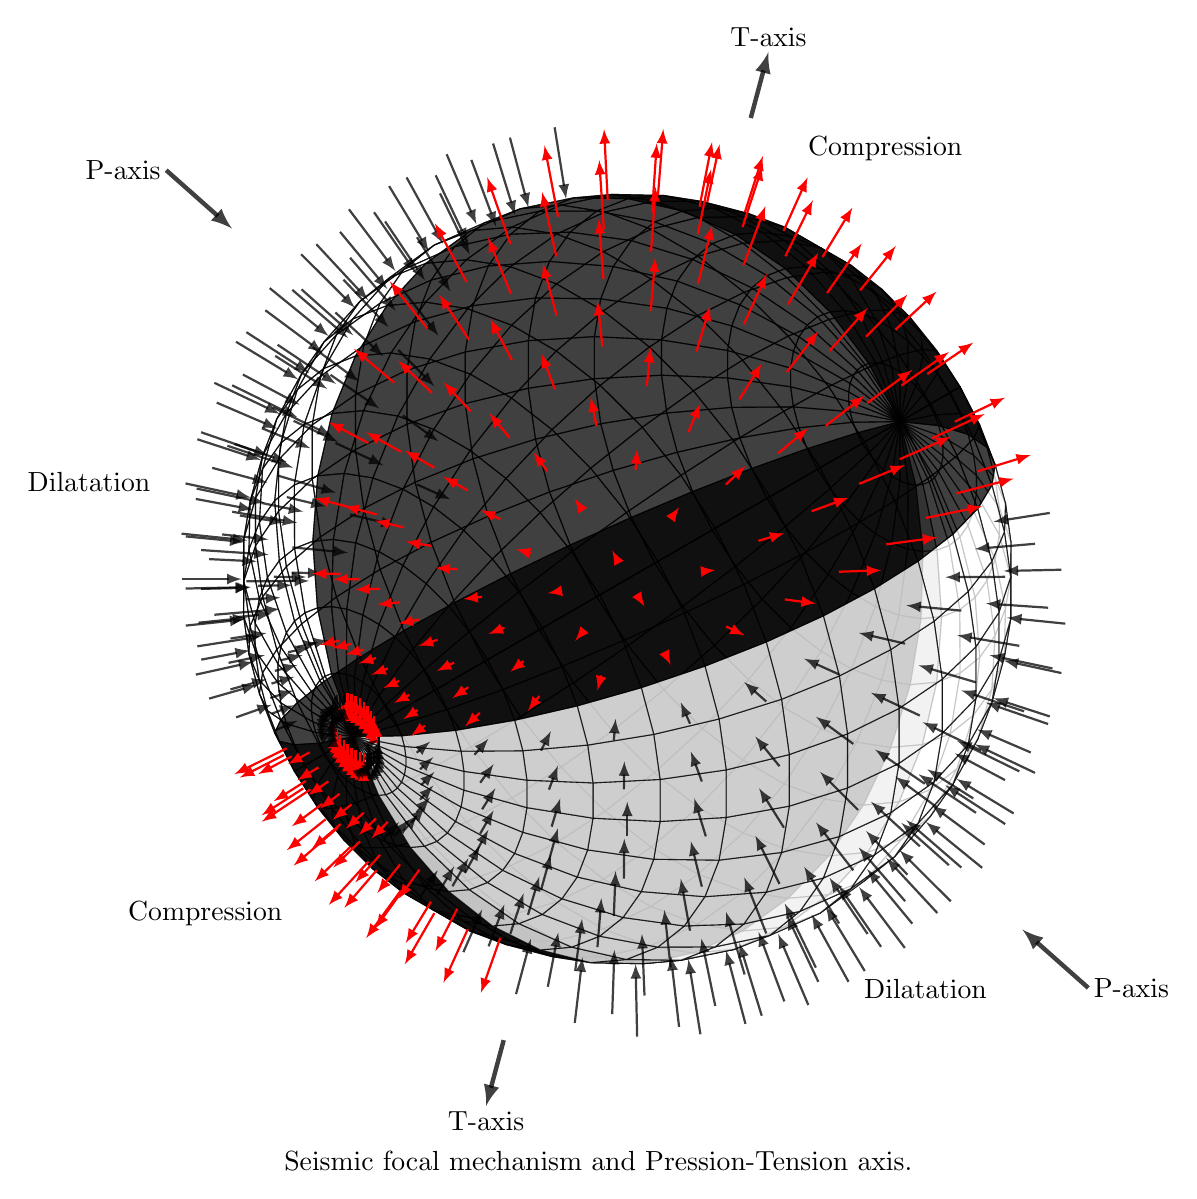
\begin{tikzpicture} [scale=4, isometricZXY, line join=round,
        opacity=.75, text opacity=1.0,%
        >=latex,
        inner sep=0pt,%
        outer sep=2pt,%
    ]
    \def\h{5}

    \newcommand{\quadrant}[2]{
        \foreach \t in {#1} \foreach \f in {175,165,...,5}
            \draw [fill=#2]
                  ({sin(\f - \h)*cos(\t - \h)}, {sin(\f - \h)*sin(\t - \h)}, {cos(\f - \h)})
               -- ({sin(\f - \h)*cos(\t + \h)}, {sin(\f - \h)*sin(\t + \h)}, {cos(\f - \h)})
               -- ({sin(\f + \h)*cos(\t + \h)}, {sin(\f + \h)*sin(\t + \h)}, {cos(\f + \h)})
               -- ({sin(\f + \h)*cos(\t - \h)}, {sin(\f + \h)*sin(\t - \h)}, {cos(\f + \h)})
               -- cycle;
    }

    %Quadrants
    \quadrant{220,230,...,300}{black}
    \quadrant{-60,-50,...,20}{white}
    \quadrant{30,40,...,120}{black}
    \quadrant{130,140,...,210}{none}

    %Movement arrows
    \foreach \t in {225,235,...,295}
        \foreach \f in {50,40,...,0}
            \draw [red, opacity=1.0, ->, thick]
                ({sin(\f - \h)*cos(\t - \h)}, {sin(\f - \h)*sin(\t - \h)}, {cos(\f - \h)})
                -- ({(1 + 0.2*cos(90 - \f))*sin(\f - \h)*cos(\t - \h)},
                    {(1 + 0.2*cos(90 - \f))*sin(\f - \h)*sin(\t - \h)},
                    {(1 + 0.2*cos(90 - \f))*cos(\f - \h)});

    \foreach \t in {125,135,...,205}
        \foreach \f in {110,100,...,0}
            \draw [black, ->, thick]
                ({(1 + 0.2*cos(90 - \f))*sin(\f - \h)*cos(\t - \h)},
                 {(1 + 0.2*cos(90 - \f))*sin(\f - \h)*sin(\t - \h)},
                 {(1 + 0.2*cos(90 - \f))*cos(\f - \h)})
                -- ({sin(\f - \h)*cos(\t - \h)},{sin(\f - \h)*sin(\t - \h)},{cos(\f - \h)});
    \foreach \t in {35,45,...,115}
        \foreach \f in {130,120,...,0}
            \draw [red, opacity=1.0 ,->, thick]
                ({sin(\f - \h)*cos(\t - \h)}, {sin(\f - \h)*sin(\t - \h)}, {cos(\f - \h)})
                -- ({(1 + 0.2*cos(90 - \f))*sin(\f - \h)*cos(\t - \h)},
                    {(1 + 0.2*cos(90 - \f))*sin(\f - \h)*sin(\t - \h)},
                    {(1 + 0.2*cos(90 - \f))*cos(\f - \h)});

    \foreach \t in {-55,-45,...,25}
        \foreach \f in {130,120,...,0}
            \draw [black, ->, thick]
                ({(1 + 0.2*cos(90 - \f))*sin(\f - \h)*cos(\t - \h)},
                 {(1 + 0.2*cos(90 - \f))*sin(\f - \h)*sin(\t - \h)},
                 {(1 + 0.2*cos(90 - \f))*cos(\f - \h)})
              -- ({sin(\f - \h)*cos(\t - \h)},{sin(\f - \h)*sin(\t - \h)},{cos(\f - \h)});

    %Annotations
    \path ({1.5*sin(100)*cos(75)}, {1.5*sin(100)*sin(75)}, {1.5*cos(100)}) node [right] {Compression};
    \path ({1.5*sin(70)*cos(-15)}, {1.5*sin(70)*sin(-15)}, {1.5*cos(70)})  node [right] {Dilatation};
    \path ({1.25*sin(50)*cos(165)},{1.25*sin(50)*sin(165)},{1.25*cos(50)}) node [left]  {Dilatation};
    \path ({1.25*sin(30)*cos(255)},{1.25*sin(30)*sin(255)},{1.25*cos(30)}) node [left]  {Compression};

    %P and T axis
    \begin{scope}[ultra thick]
        \draw[->] ({1.75*sin(90)*cos(75)}, {1.75*sin(90)*sin(75)}, {1.75*cos(90)})
            -- ({2*sin(90)*cos(75)},{2*sin(90)*sin(75)},{2*cos(90)}) node [above] {T-axis};
        \draw[->] ({1.75*sin(90)*cos(255)},{1.75*sin(90)*sin(255)},{1.75*cos(90)})
            -- ({2*sin(90)*cos(255)},{2*sin(90)*sin(255)},{2*cos(90)}) node [below] {T-axis};
        \draw[<-] ({1.5*sin(90)*cos(-15)}, {1.5*sin(90)*sin(-15)}, {1.5*cos(90)})
            -- ({1.75*sin(90)*cos(-15)},{1.75*sin(90)*sin(-15)},{1.75*cos(90)}) node [right] {P-axis};
        \draw[<-] ({1.5*sin(90)*cos(165)}, {1.5*sin(90)*sin(165)}, {1.5*cos(90)})
            -- ({1.75*sin(90)*cos(165)},{1.75*sin(90)*sin(165)},{1.75*cos(90)}) node [left] {P-axis};
    \end{scope}

    % Label
    \node [anchor=north, yshift=-2mm] at (current bounding box.south)
        {Seismic focal mechanism and Pression-Tension axis.};
\end{tikzpicture}
\end{document}